\section{State of the Art / Background }
	% todo a summary of the newest techniques and inventions in the field
	% of twitter research related to finance. 

\subsection{Twitter}
Twitter is a social and information networking. It's a real-time service that
connects users to the latest stories, their interests, ideas and much more. The
microblogging site allows users to find and follow accounts that the user has
an interest in. 

At the core of Twitter you have the Tweet. The Tweet is the 140 character
message. These bursts of information combined are the life blood of Twitter.
Tweets lets you communicate with other users, share photos, post all kinds of
information. The small size of the tweets are not a hindrance for the flow of
information. 
\footnote{About Twitter: \url{https://twitter.com/about}}

The fast growing messaging service handles 1.6 billion searches every day.
As of 2012 the 500 million users would generate 3.2 queries each on any given
day. 340 million tweets were posted every day. 
\footnote{Wikipedia: \url{http://en.wikipedia.org/wiki/Twitter}} 

Most medium and large companies have a presence on Twitter today. Posts can contain
any type of information, from promotional content to service status to
financial reports. \cite[p8]{annikajubbega11:twitter_driver_stock_price} says
that 77 of the Fortune 100 companies have a twitter account. 

Companies use twitter for feedback and customer relations. Questions can be
asked with a hashtag of to a specific user. This makes it easy to sort filter
the messages, and therefore easier to get in contact with the customer. Best
Buy demonstrated the successfulness of twitter in customer relations by
answering questions with a specific hashtag. In 2009 they had answered nearly
20 thousand questions using twitter. \cite[p1]{Li2013206}
Market Intelligence is also a major aspect of the microbloggin sphere.

Twitter represents one of the largest and most dynamic datasets of user
generated content. Along with Facebook twitter data is real time. This has major
implications for anyone who are interested in sentiment, public opinion or
customer interaction. \cite[]{sperious11}

A typical tweet contains about 11 words and provides an opinion or state of
mind or a piece of information. Tweets can contain hashtags: #something, user:
@username, or other adaptations of prefixes such as \$STO which represents a
stock. The different prefixes or tags (\$, \#, @) easily distinguishes the
content of the tweet. This also makes it easier to search and classify the
content of tweets. Examples of tweets can be found in figure:\ref{fig:sto} and
figure:\ref{fig:tweet1}.

The retrieval of tweets seems like a challenge and practically impossible with
a web scraper. But Twitter has made this easy by providing an API
\footnote{API: Application programming interface}. With the API you can write
tweets and update the status of a user. But the best part of the API is that it
provides search capabilities. To get a certain subset of all tweets, we can use
the search function and view only the tweets we want. 

On the front page of twitter we have the search function at the top right of
the page. The search provides the ability to limit the tweets you look at and
gives you the opportunity to find the information you are looking for. 

\begin{figure}[htb]
    \centering
    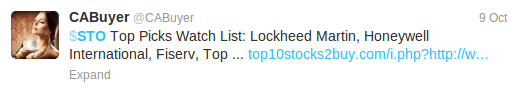
\includegraphics[width=\textwidth]{STO} 
    \caption{Typical tweet from Twitter.}
    \label{fig:sto}
\end{figure}

%\begin{figure}[htb]
%    \centering
%    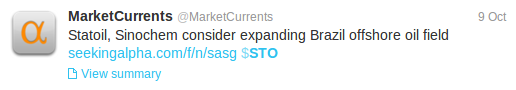
\includegraphics[width=\textwidth]{STO2} 
%    \caption{The text that shows under the image, image text.}
%    \label{fig:sto2}
%\end{figure}

\begin{figure}[htb]
    \centering
    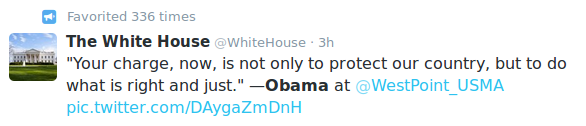
\includegraphics[width=\textwidth]{tweet1} 
    \caption{Typical tweet from Twitter.}
    \label{fig:tweet1}
\end{figure}

%\begin{figure}[htb]
%    \centering
%    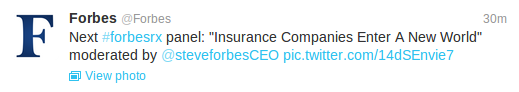
\includegraphics[width=\textwidth]{tweet2} 
%    \caption{The text that shows under the image, image text.}
%    \label{fig:tweet2}
%\end{figure}
%
%\begin{figure}[htb]
%    \centering
%    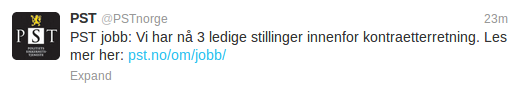
\includegraphics[width=\textwidth]{tweet3} 
%    \caption{The text that shows under the image, image text.}
%    \label{fig:tweet3}
%\end{figure}

\subsection{Sentiment}

Opinion mining on the web is not a new phenomenon. But in resent years it has
become much more attractive to traders in the financial world. Twitter and the
social media's opinion is on the rise. This means a surplus of raw data with
easy access. Companies all over the world has started to use twitter and
readily available tweets to their benefit. Trading with social media is part of
the trend. Although there are some drawbacks and shortcomings. Noise and
garbage is one of them. It's difficult to accurately sort through all the data
and get only the information relevant for your use. Even if you're right 80\% of
the time, the last 20\% can prove devastating.
\cite[]{stevenson12:social_media_stock_pickers}

Sentiment broadly refers to the state of mind a person has. Whereas negative or
positive. Based on the current state of mind the person will do optimistic or
pessimistic choices. A positive state of mind leads to optimistic judgements of
future events. And a negative state of mind leads to pessimistic judgements.
\cite[p4]{doukas10:sentiment_and_momentum}

The intention of users are also a part of the driver in user activity on
microbloggs. The users may have different roles and intentions in different
communities in the microblogging sphere, \cite[]{java07}. This might also be a
factor in the sentiment analysis.

\subsubsection{Sentiment Analysis}

% todo This should be present: 
% methods used
	% adding features to the tweet.
	% Lexicon, positive / negative.
	% labeled graph propagation.
% tagging of words 

\cite[]{Li2013206} approaches the classification of sentiment in tweets in four
steps. First is the topic detection. The topic is the overall theme of the
message. This step extracts and identifies the topics associated with the
queries of users. Following that the classification of opinion happens. This
judges the polarity of the sentiment. The state of mind of the user can be
recorded.

A problem that arises is the credibility of the expresser. \cite[]{Li2013206} addresses this to
get a better summary of the sentiment. Then aggregates, the
three previously described parts of the classification, to get a truer
reflection of the opinions.

\cite[]{barbosa10} looks upon the problem of noise in biased and noisy data. 
They focus on noisy labels and add features to the tweets to increase the
classification properties of the tweets. Then the tweets are classified as
subjective or objective. This is to filter out the tweets that don't project a
sentiment. The subjective tweets are then classified as positive or negative.
Then \cite[]{barbosa10} generalise the classification of tweets by using meta
data about the tweets and how tweets are written. This results in a more
abstract representation of tweets and the classification. \cite[]{barbosa10}
provides a better way to classify tweets.

Another approach to the sentiment challenges with twitter is explored by
\cite[]{becker13}. Their explorations techniques for Contextual Polarity Disambiguation
and Message Polarity Classification. Constrained and supervised learning is
used to create models for classification. They describe a system that solves
these tasks with the help of polarity lexicons and dependency parsers. 
Expanded vocabulary is one of the main aspects of their success, as they say in
their findings: "We hypothesize this performance is largely due to the expanded vocabulary
obtained via unlabeled data and the richer syntactic context captured with
dependency path representations." \cite[]{becker13}

Earlier \cite[]{sperious11} have researched the polarity classification of tweets. 
In contrast to \cite[]{becker13}, \cite[]{sperious11} has used distant
supervision and labeled propagation on a graph based data structure. The data
structure represents users with tweets as nodes. And tweets with bigrams,
unigrams, hashtags, etc as subnodes of the tweets. A label propagation approach
rivals a model supervised with in-domain annotated tweets and outperforms the
noisily supervised classifier and a lexicon-based polarity ratio classifier.
\cite[]{sperious11} 

\subsubsection{Sentiment in Finance}
\cite[p2]{Brown20041} writes the following on over-reaction of investors: "
He(Siegel (1992)) concludes that shifts in investor sentiment are correlated
with market returns around the crash. Intuitively, sentiment represents the
expectations of market participants relative to a norm: a bullish (bearish)
investor expects returns to be above (below) average, whatever ‘‘average’’ may
be.". In the light of resent changes in the financial world and the use
of sentiment from social media, the notion that opinions and sentiment of
investors and market actors affect the market is not a new observation.

Use of sentiment can predict changes and momentum in the market.
Bad news in an optimistic period creates cognitive dissonance in the small
investors. This impacts the market by slowing down the selling rate of loosing
stocks. \cite[p29]{doukas10:sentiment_and_momentum}

Further we can see that optimistic sentiment has a 2\% monthly average return.
While the investor sentiment is pessimistic we see a drastic reduction in
returns. Down to 0.34\%,\cite[p5]{doukas10:sentiment_and_momentum}.
After optimistic periods it is indicated that the monthly return is reduced to
-0.49\%. On the contrary there is no equivalent change after a pessimistic
period, \cite[p6-7]{doukas10:sentiment_and_momentum}.
Momentum profits are only significant when the sentiment is optimistic,
\cite[p29]{doukas10:sentiment_and_momentum}.

Hope and fear is used by \cite[]{Zhang201155} to decide the movement of the
market. The sentiment is aggregated to be hopeful or fearful. This basically
focuses on positivity and negativity of the sentiment of that particular day.
The daily sentiment is then compared to the market indicators of the same day
to create a prediction of the market. \cite[]{Zhang201155} finds that calm
times give little hope or other emotions. Little turmoil results in few
fluctuations in the market. And opposite, lots of emotions(hope, worry, fear),
gives speed to the market.

\cite[p3]{Brown20041} indicates that the sentiment does not cause subsequent
market returns. For a short-term marketing timing this is bad news. However
with the changes in social media over the last decade how is the situation
today? With the microblogging sphere of today we can easily see the
correlation of sentiment and the market indicators,
\cite[]{annikajubbega11:twitter_driver_stock_price}. But
does the sentiment cause changes in the market-return?
\cite[p3]{Brown20041} also says that optimism is associated with overvaluation
and subsequent low returns.

\cite[p]{Brown20041} concludes that aggregated sentiment measures has strong
co-movement with changes in the market. He also indicates that sentiment
doesn't appear to be a good trading strategy. This, in the view of
\cite[]{Zhang201155}, indicates a leap in sentiment research and what is possible
with the microblogging of today.

\subsection{Finance and Trading}
%Finance and Trading on and with twitter. 
%\cite[p.2]{annikajubbega11:twitter_driver_stock_price}

%Sites like \href{http://stocktwits.com}{StockTwits.com}

The management of assets or liabilities and the management of funds over a
period of time is called Finance. In finance the valuation of assets are time
dependant. The same asset is not worth the same now and in a few minutes. Assets are
priced based on expected returns and risk level. The three sub categories of
finance are: personal, corporate and public. 
\footnote{Wikipedia:\url{http://en.wikipedia.org/wiki/Finance}}.
These categories describes very different parts of the financial world. 

Trading is the action of buying or selling financial instruments.
Financial instruments can be stocks, bonds, derivatives or commodities 
\footnote{Wikipedia:\url{http://en.wikipedia.org/wiki/Trader_(finance)}}.
Trades takes place in markets,  stock markets, derivatives markets or commodity
markets.

Personal finance touches on the problems of handling the funds to make ends
meet in your personal life. This can be things like tax policies, pension
funds, heirlooms etc. Personal finance has a big element of economy. This is
the control of income and expenses and the ending result of your total usage of
money.  

Corporate finance deals more in terms of investments over time and the
financial position of assets to generate the maximum revenue. This is more of a
strategic game of money placement and capital management. 

The public finance are the money countries and states use. The finance related
to sovereign and sub-national entities
\footnote{Wikipedia:\url{http://en.wikipedia.org/wiki/Finance#Public_finance}}.
National banks and the production of money are also categorised under this
category.

% todo write about technical analysis. 
Technical analysis in finance. 


\subsection{The Trend}
The trend is the general opinion of the masses. As defined by the Free
Dictionary:  
"The direction and momentum of a market, price, economy, or other measure. For
example, if the price of a security is going mainly downward with only a few
gains here and there, it is said to be on a downward trend. Identifying and
predicting trends is important to finding the right moment to buy and sell
securities. Trends are especially important in technical analysis, which
recommends buying at the bottom of a downward trend and selling at the top of an
upward trend."
\footnote{Dictionary description of trend: \url{http://financial-dictionary.thefreedictionary.com/Trend}}

It's often talk about the fashion trend or the music trend when regular people
talk about the trend. Or just the general direction of which a subject or
subculture are moving. 

Trends work in much the same way as opinions on any other ting. One person
comes first and says something. Then others start to think the same thing or
feel the same way. The first group of people that move in the same direction
are called trend setters. They are the people that show others how this trend works and
what this trend is about. 

On twitter we have lots of subcultures that all express themselves on their
specific topic. Whether it's technology, art, finance or any other thing.  
In the sense of twitter we can take a step back and look at the content of
messages and from there see if we can find common topics that people talk
about, this being the topic of a subculture or a subspace of twitter. To get
the trend we have to look at the content of the messages in a subspace. Given
that the trend is the collective general collective opinion of the subspace we
can look into this an see if we can find certain topics or areas of interest
that aggregates to a trend. 

When looking for twitter and trends there are few of far between those who work
on it. No material or indication is found to suggest that trending on twitter
is researched in regards to sentiment analysis of tweets.


